%\documentclass[10pt,conference]{IEEEtran}
\documentclass[sigconf,screen]{acmart}

% correct bad hyphenation here
%\hyphenation{op-tical net-works semi-conduc-tor}

% !TEX root =  paper.tex

% \usepackage{cite}
% \usepackage{amsmath,amssymb,amsfonts}
% \usepackage{algorithmic}
% \usepackage{graphicx}
% \usepackage{subcaption}
% \usepackage{textcomp}
% \usepackage{xcolor}
% \usepackage{multicol} % \columnbreak
% \usepackage{balance}
% \usepackage{enumitem}    
%\usepackage[table]{xcolor}
%\usepackage{nohyperref}

\usepackage{xcolor}

\usepackage{tabularx} 
\usepackage{collcell}

% \usepackage[usenames,dvipsnames,svgnames,table,xcdraw]{xcolor}
% \usepackage[usenames,dvipsnames,svgnames]{xcolor}
% \usepackage{pgfplots}
% \pgfplotsset{compat=1.10}


\usepackage{booktabs}
\usepackage[caption=false,font=normalsize,labelfont=sf,textfont=sf]{subfig}
%\usepackage{cite}
% \usepackage{hyperref}
\usepackage{array}
\usepackage{threeparttable}
\usepackage{enumitem}    
\usepackage[greek,english]{babel}
\usepackage{ifthen}
\usepackage{xspace}
\usepackage{fancybox}
\usepackage{marginnote}
\usepackage{tcolorbox}
\usepackage{multirow}
\usepackage{mathtools}
\usepackage{algpseudocode, algorithm, algorithmicx}
\usepackage{color}
\usepackage{soul}
\usepackage{graphicx}
\usepackage{amsmath}
\usepackage{tikz}
\usepackage{cleveref}
\usepackage{hhline}
\usepackage{balance}

\usepackage{listings}
\usepackage{parcolumns}
\usepackage{cleveref}

\usepackage{array}

\usepackage{adjustbox}
\usepackage{flushend}
\usepackage[switch]{lineno}
\definecolor{light-gray}{gray}{0.95}
\newcommand{\code}[1]{\colorbox{light-gray}{\fontsize{9pt}{10pt}\texttt{#1}}}

\definecolor{circled-color}{gray}{0.15}
\newcommand*\circled[1]{\tikz[inner sep=.1ex,baseline=-.75ex] \node[circle,draw,color=white,fill=circled-color] {#1};}


\def\BibTeX{{\rm B\kern-.05em{\sc i\kern-.025em b}\kern-.08em
    T\kern-.1667em\lower.7ex\hbox{E}\kern-.125emX}}
\newboolean{showcomments}
\setboolean{showcomments}{true}
\hypersetup{draft,bookmarks=false}

\ifthenelse{\boolean{showcomments}}
{
	\definecolor{myyellow}{RGB}{255, 228, 26}
	\definecolor{myblue}{RGB}{50, 50, 220}
	\newcommand{\nb}[2]{
		{\sf
			\fcolorbox{myyellow}{yellow}{\scriptsize\textbf{#1}}%
			$\blacktriangleright$%
			{\color{myblue}\fontsize{7pt}{8pt}\selectfont\textbf{#2}}%
		}%
	}
}
{
	\newcommand{\nb}[2]{}
}


\newcommand{\Mo}[1]{\nb{Mo}{#1}}
\newcommand{\Ali}[1]{\nb{Ali}{#1}}


\usepackage{color}


\definecolor{editorGray}{rgb}{0.95, 0.95, 0.95}
\definecolor{editorOcher}{rgb}{1, 0.5, 0} % #FF7F00 -> rgb(239, 169, 0)
\definecolor{editorGreen}{rgb}{0, 0.5, 0} % #007C00 -> rgb(0, 124, 0)

\lstdefinelanguage{JavaScript}{
  morekeywords={typeof, new, true, false, catch, function, return, null, catch, switch, var, if, in, while, do, else, case, break},
  morecomment=[s]{/*}{*/},
  morecomment=[l]//,
  morestring=[b]",
  morestring=[b]'
}
\lstdefinelanguage{HTML5}{
        language=html,
        sensitive=true, 
        alsoletter={<>=-},
        otherkeywords={
        % HTML tags
        <html>, <head>, <form>, </form>, <div>, </div>, <p>, </p>, 
        <span>, </span>, <input, <textarea, </textarea>, <select, </select>, 
        <option>, </option>, <title>, </title>, <meta, />, </head>, <body>,
        <canvas, \/canvas>, <script>, </script>, </body>, </html>, <!, html>, <section>, </section>
        },  
        ndkeywords={
        % General
        =,
        % HTML attributes
        charset=, id=, width=, height=, type=, value=, checked
        % CSS properties
        border:, transform:, -moz-transform:, transition-duration:, transition-property:, transition-timing-function:
        },  
        morecomment=[s]{<!--}{-->},
        tag=[s]
}

\lstdefinelanguage{CSS}{
  morekeywords={background,color,display,justify,content,font,weight,border,size,padding},
  morestring=[s]{:}{;},
  sensitive,
  morecomment=[s]{/*}{*/}
}
\newcommand{\todo}[1]{\textcolor{magenta}{\nb{TODO:}{#1}}}
\newcommand{\header}[1]{\par\smallskip\noindent\textbf{#1.}}
\newcommand{\toolname}{\textsc{AxeForm}\xspace}
\newcommand{\html}{\textsc{HTML}\xspace}
\newcommand{\css}{\textsc{CSS}\xspace}
\newcommand{\javascript}{\textsc{JavaScript}\xspace}
\lstset{%
    % Basic design
    backgroundcolor=\color{editorGray},
    basicstyle={\linespread{1.0}\scriptsize\ttfamily},   
    frame=l,
    % Line numbers
    xleftmargin={0.75cm},
    numbers=left,
    stepnumber=1,
    firstnumber=1,
    numberfirstline=true,
    % Code design   
    keywordstyle=\color{blue}\bfseries,
    commentstyle=\color{darkgray}\ttfamily,
    ndkeywordstyle=\color{editorGreen}\bfseries,
    stringstyle=\color{editorOcher},
    % Code
    language=HTML5,
    alsolanguage=JavaScript,
    alsodigit={.:;},
    tabsize=2,
    showtabs=false,
    showspaces=false,
    showstringspaces=false,
    extendedchars=true,
    breaklines=true,        
    % Support for German umlauts
    literate=%
    {Ö}{{\"O}}1
    {Ä}{{\"A}}1
    {Ü}{{\"U}}1
    {ß}{{\ss}}1
    {ü}{{\"u}}1
    {ä}{{\"a}}1
    {ö}{{\"o}}1
}






%%% The following is specific to ASE '18 and the paper
%%% 'Generating Reusable Web Components from Mockups'
%%% by Mohammad Bajammal, Davood Mazinanian, and Ali Mesbah.
%%%
\setcopyright{acmcopyright}
\acmPrice{15.00}
\acmDOI{10.1145/3238147.3238194}
\acmYear{2018}
\copyrightyear{2018}
\acmISBN{978-1-4503-5937-5/18/09}
\acmConference[ASE '18]{Proceedings of the 2018 33rd ACM/IEEE International Conference on Automated Software Engineering}{September 3--7, 2018}{Montpellier, France}
\acmBooktitle{Proceedings of the 2018 33rd ACM/IEEE International Conference on Automated Software Engineering (ASE '18), September 3--7, 2018, Montpellier, France}


%\copyrightyear{2018} 
%\acmYear{2018} 
%\setcopyright{acmcopyright}
%\acmConference[ASE '18]{33rd ACM/IEEE International Conference on Automated Software Engineering}{September 3--7, 2018}{Montpellier, France}
%\acmBooktitle{33rd ACM/IEEE International Conference on Automated Software Engineering (ASE '18), September 3--7, 2018, Montpellier, France}
%\acmPrice{15.00}
%\acmDOI{10.1145/3238147.3238194}
%\acmISBN{978-1-4503-5937-5/18/09}


\begin{document}

\title{Generating Reusable Web Components from Mockups}

%% ACM ART Author format
%\author{Mohammad Bajammal}
%\email{bajammal@ece.ubc.ca}
%\author{Davood Mazinanian}
%\email{dmazinanian@ece.ubc.ca}
%\author{Ali Mesbah}
%\email{amesbah@ece.ubc.ca}
%\affiliation{ 
%	\institution{University of British Columbia}
%	\city{Vancouver, BC} 
%	\country{Canada}
%}


%\author{Mohammad Bajammal}
%\affiliation{ 
%	\institution{University of British Columbia}
%	\city{Vancouver, BC} 
%	\country{Canada}
%}
%\email{bajammal@ece.ubc.ca}
%
%
%\author{Davood Mazinanian}
%\affiliation{ 
%	\institution{University of British Columbia}
%	\city{Vancouver, BC} 
%	\country{Canada}
%}
%\email{dmazinanian@ece.ubc.ca}
%
%
%\author{Ali Mesbah}
%\affiliation{ 
%	\institution{University of British Columbia}
%	\city{Vancouver, BC} 
%	\country{Canada}
%}
%\email{amesbah@ece.ubc.ca}



\author{Mohammad Bajammal}
\affiliation{
 \institution{University of British Columbia}
 \streetaddress{2332 Main Mall}
 \city{Vancouver, BC}
 \country{Canada}
 \postcode{V6T 1Z4}
}
\email{bajammal@ece.ubc.ca}

\author{Davood Mazinanian}
\affiliation{
 \institution{University of British Columbia}
 \streetaddress{2332 Main Mall}
 \city{Vancouver, BC}
 \country{Canada}
 \postcode{V6T 1Z4}
}
\email{dmazinanian@ece.ubc.ca}

\author{Ali Mesbah}
\affiliation{
 \institution{University of British Columbia}
 \streetaddress{2332 Main Mall}
 \city{Vancouver, BC}
 \country{Canada}
 \postcode{V6T 1Z4}
}
\email{amesbah@ece.ubc.ca}



\begin{abstract}

Filling web forms is a common online activity. 
Web forms are made accessible to users with disabilities 
by conveying their content through specific DOM labeling 
markups. The absence of these markups is one of the most 
common accessibility errors. However, there is currently 
little to no work in terms of having an automated analysis 
process that allows inferring the labeling markups in order 
to automatically make forms accessible for users with disabilities. 
In this paper, we propose a web form analysis approach that 
infers labels by first constructing different types of 
visual cues from a form, then optimizing the combination of 
various cues and form fields, and finally augmenting the DOM 
to incorporate the required labeling markup. We evaluate 
our approach on real-world subjects and assess the accuracy 
of labeling inference, the safety of the DOM augmentation, 
as well as the labeling performance. The results show an 
average F1-measure of 88.4\% for label inference, and an 
average run-time of around 1.6 seconds.

\end{abstract}

\keywords{web forms, accessibility errors, 
accessibility repair, visual analysis}



\begin{CCSXML}
<ccs2012>
<concept>
<concept_id>10011007.10011074.10011092</concept_id>
<concept_desc>Software and its engineering~Software development techniques</concept_desc>
<concept_significance>300</concept_significance>
</concept>
<concept>
<concept_id>10011007.10011074.10011092.10010876</concept_id>
<concept_desc>Software and its engineering~Software prototyping</concept_desc>
<concept_significance>300</concept_significance>
</concept>
</ccs2012>
\end{CCSXML}

\ccsdesc[300]{Software and its engineering~Software development techniques}
\ccsdesc[300]{Software and its engineering~Software prototyping}



\keywords{web UI, web components, web refactoring, machine learning, computer vision}

% make the title area
\maketitle



% !TEX root =  paper.tex

\section{Introduction}
\label{section:introduction}

The development of user interfaces (UIs) for web apps is often a manual and time 
consuming task.In a survey of more than 5,700 developers, 51\% reported working 
on app UI design tasks on a daily basis~\cite{IDC:survey},
more so than other development tasks, which they tended to perform every few days. 
Another study also showed that an average of 48\% of the code size of software is 
related to the user interface~\cite{myers:ui:survey}.

A common workflow for creating web user interfaces 
is \textit{mockup based design}~\cite{Newman:2000:SitemapsStoryboardsSpecifications, Ozenc:2010:SupportDesigners}.
In this approach, a graphic designer creates a rough illustration of the anticipated UI design, called the \textit{mockup} or \textit{wireframe},
usually through a graphic design software or a WYSIWYG editor. 
This mockup is then exported to \html to be rendered in a browser.
A web developer then examines the mockup and begins constructing web components for the app, which are nowadays implemented in one of the popular front-end frameworks such as \angular~\cite{Angular} or \react~\cite{React}.

\renewcommand{\toolname}{\textsc{VizMod}\xspace}
The main building block of UI design, and a cornerstone of these front-end frameworks, is the concept of  
\textit{reusable components}~\cite{React-components, Angular-components},
which are a set of APIs and coding practices allowing reuse and encapsulation of repeated patterns on the front-end.
Reusable components help improve modularity and maintainability, make the code more testable, and effectively remove duplication,
by offloading the task of creating repetitive patterns to the web browser at runtime. 
Recent surveys show that using front-end frameworks is extensively popular among web developers. In one survey more than 92\% of around 28,000 surveyed web developers stated that they use a framework 
rather than constructing UIs using pure \html~\cite{StateOfJS:WebPlatformTests}.
As a result, creating reusable components is often an essential element of building an app's front-end.

This component creation process can often be time consuming and tedious~\cite{thinking:in:components} in practice;  
 it requires several manual steps,
including the examination of the mockup, 
checking potential elements that may or may not be suitable for conversion to components, 
constructing a template for components that unifies repeated segments, 
adding placeholders for variable content, and
refactoring the code to replace instances with instantiated components~\cite{thinking:in:components}.

To the best of our knowledge, there has been little to no automated support in creating these reusable web components from mockups. Existing techniques help to manage mockups themselves, but do not generate any components. For instance, one set of approaches~\cite{Sinha:2013:CompilingMockupsToFlexibleUIs, ramon2016layout} takes a mockup as input
and converts its layout into a responsive code (e.g., through CSS) such that it is flexible  to maintain the layout on different
display sizes. Others~\cite{mihalcea2014const_with_mockups} propose a tool that overlays the mockup as a transparency layer while implementing the UI, 
and performs a snapping-like functionality that aligns against various parts of the mockup.

In this chapter, we propose a technique, implemented in a tool, \toolname, to fill this gap by automatically generating reusable web components from mockups.
Given a web mockup, our technique automatically identifies patterns on the UI,  refactors the \html code, and creates reusable components for popular front-end frameworks that are already familiar to developers such as \react or \angular. At the core of our approach is an unsupervised machine learning process for the detection of reusable UI patterns; we use features composed of a hybrid of information obtained from the Document Object Model (DOM) 
as well as the visual analysis of the UI.

We evaluate \toolname on \numberOfTemplates real-world web mockups by automatically identifying and transforming \totalNumberOfComponentInstances component instances 
into \numberOfComponents components.    
We also ask \numberOfParticipants experts to manually
find patterns on the mockups
and compare the output from our approach with the manually-identified patterns.
Our approach is able to achieve \precision precision and \recall recall, on average, in correctly detecting reusable patterns in the UIs. 


This chapter makes the following main contributions:
\begin{itemize}
	\item A novel approach for automatically generating web components (e.g., \react, \angular) from mockups, which is the first to address this issue, to the best of our knowledge.
	\item An implementation of our approach, available in a tool called \toolname.
	\item A qualitative and quantitative evaluation of \toolname in terms of its accuracy and reusability of the generated components. 
	
\end{itemize}


 




\begin{figure}
    \noindent
	\begin{minipage}[c]{.97\columnwidth}
        \centering
        \begin{lstlisting}[language={HTML5},frame=ltbr,aboveskip=1.1em,basicstyle={\linespread{1.0}\footnotesize\ttfamily},]
<form>
<section>
 <div><p>Name</p></div>
 <div><p>Business Email</p><span>free providers not accepted</span></div>
</section>
<input type="text" id="vr_9481">
<textarea id="bx_3978"></textarea>
<input type="text" id="vr_6588">
<div><p>Message</p></div>
<section>
 <div><p>Do you have an open ticket?</p></div>
 <div><p>How often should we email you?</p></div>
 <span>Yes</span><span>No</span>
</section>
<input type="radio" value="Y" id="op_y">
<input type="radio" value="N" id="op_n" checked>
<select id="frq"><option>daily</option>
 <option>weekly</option><option>monthly</option>
</select>
</form>
        \end{lstlisting}
    (a) Sample of the HTML markup
    \end{minipage} \hfill
	\begin{minipage}[c]{\columnwidth}
        \centering
        \fbox{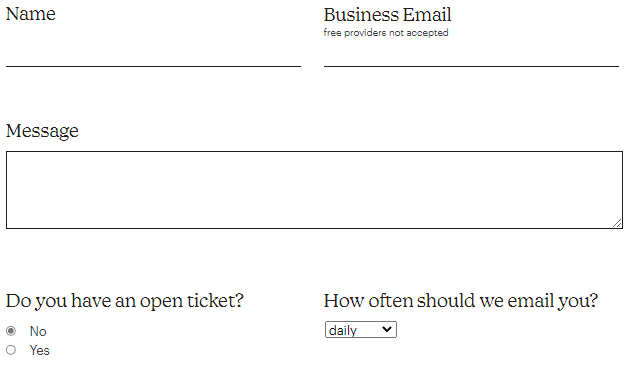
\includegraphics[width=\linewidth]{accessibility_repair/figures/motivating-example/rendered.png}}
        (b) Rendered form
    \end{minipage}
%	\begin{minipage}[c]{.98\columnwidth}
%	\centering \ \\
%	(a) Sample of the HTML markup
%	\end{minipage}
%	\begin{minipage}[c]{.98\columnwidth}
%	\centering \ \\
%	(b) Rendered form
%	\end{minipage}
	\ \\ \caption{An example of an inaccessible web form.}
    \label{fig:motivating-example}
  \end{figure}

% !TEX root =  paper.tex
\section{Approach}

In this chapter, we propose an approach to
automatically test for a subset of web accessibility violations 
that are pertinent to semantic structure.
We recall that the scope of this work focuses on  
vision disabilities as opposed to other forms of disability, 
due to the web being a predominantly visual medium 
and the fact that vision disabilities 
are the most common software-related disability~\cite{2019users_survey}. 

\Cref{fig:approach} shows an overview of our 
proposed approach, which is based on the strategy of visually 
analyzing the web page to infer semantic groupings and their roles, 
and then checking that the HTML markup matches the inferred semantic roles.
The approach begins by obtaining the Document Object Model (DOM)
and screenshot of the web page rendered in a web browser.
Next, the set of visibly perceivable objects is identified.  
This is then used to perform a semantic grouping of the page into 
a set of semantically coherent regions. 
Subsequently, this information is used in an 
inference stage where the specific semantic role 
of each region is detected.
Finally, the inferred semantics are checked against the markup
used in the page, and a report is generated as to which 
parts of the page are inaccessible.
The rationale behind this strategy is to check whether 
  the semantics visually perceivable by sighted 
users are reflected in the semantics of the HTML markup,
thereby ensuring accessibility. 

\begin{figure}[t]
    \centering
    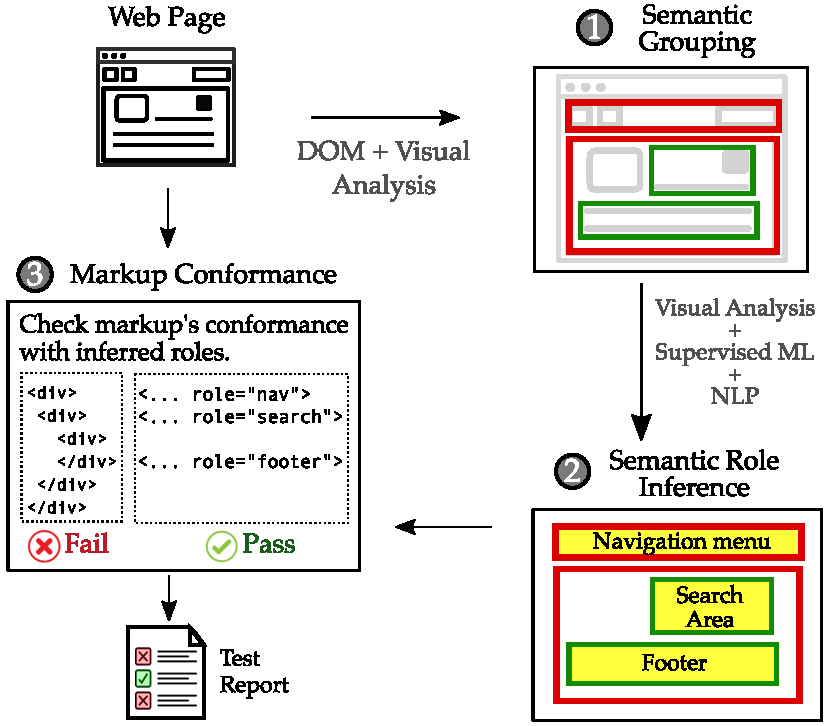
\includegraphics[width=0.7\linewidth]{accessibility_testing/figures/approach/approach.pdf}
    \caption{Overview of the proposed approach.}
    \label{fig:approach}
\end{figure}

\subsection{Visual Objects Identification}
In this first stage,
the goal is to identify objects that 
are perceivable by sighted users, which we refer to as \emph{\vizobjs}. 
For instance, in \Cref{fig:motivating-example}(c), 
each item in the top navigation menu would be a {\vizobj}. 
This step of visual objects identification is the 
foundation of our overall approach, 
since the identification of {\vizobjs} enables checking whether the information
and elements that are perceivable by sighted users 
are also accessible to non-sighted users. 
 

\subsubsection{Objects Extraction}\label{subsec:extraction}

We begin by taking as input the DOM of the page 
after it is loaded and rendered in a browser. We 
then extract from the DOM a set of nodes that 
represent visual content of the page, 
and we refer to each of these as \emph{{\VizObjs}}.
We define three types of {\VizObjs}:
textual, image, and interactive.

\header{Textual Objects}
The extraction of text content is achieved by 
traversing text nodes of the DOM. More specifically:
\begin{align}
    \Theta_{t} \coloneqq \{ E \:\vert\: \nu(E) \land \tau(E) \}
\end{align}
where $\Theta_{t}$ is the set of all {\vizobjs} that represent text in the page,
$E \in DOM$ is a leaf element iterator of the rendered DOM in the browser,
$\nu(E)$ is a heuristic predicate that runs a series of checks
to detect visually perceivable elements (as will be described in \cref{subsub:vizassert}),
and $\tau(E)$ is a predicate that examines whether
there is a text associated with $E$. 
More specifically, it returns
non-empty nodes of DOM type \code{\#TEXT},
which represent string literals. 
An example of extracted textual objects would be the ``Resources'' section in 
\Cref{fig:motivating-example}(c).
We note that the predicate is based on a node type, rather than
an element (i.e., tag) type.
This allows more robust abstraction because the predicate captures any text and does not
make assumptions about how developers choose to place their text.
In other words, regardless of the tag used for text data (e.g., \code{<span>, <div>}),
text would still be stored in nodes of type \code{\#TEXT}, even for custom HTML elements.
This helps in making the approach more robust by reducing assumptions about
tags and how they are used in the page.

\header{Image Objects}
Subsequently, we perform another extraction for image objects.
We define this as follows:
\begin{align}
    \Theta_{m} \coloneqq \{ E \:\vert\: \nu(E) \land \mu(E) \}
\end{align}
where $\Theta_{m}$ is the set of all objects that are present in the page and represent images.
As in the previous case,
the predicate $\mu(E)$ examines whether
there is any relevant image content associated with $E$.
This has two possibilities:
a) nodes of \code{<img>}, \code{<svg>}, and \code{<canvas>} elements, 
and b) non-image nodes with a non-null background image.
An example of extracted image objects would be the bell icon in 
\Cref{fig:motivating-example}(c).
We note that this predicate makes the proposed approach more robust
by eliminating assumptions about how developers markup images. 
If images are contained in standard tags (e.g., \code{<img>}, \code{<svg>}),
then the predicate readily captures them. 
However, we make no assumptions that this is the only way an image can be included.
For this reason, we also capture elements of any type when a non-null background image 
is detected.

\header{Interaction Objects}
Finally, we extract the interaction elements as follows:
\begin{align}
    \Theta_{i} \coloneqq \{ E \:\vert\: \nu(E) \land \eta(E) \}
\end{align}
where $\Theta_{i}$ is the set of all {\vizobjs} that represent form elements 
or similar interactive elements.
These are determined by the predicate $\eta(E)$, which collects
elements such as input fields and drop down menus.
An example of extracted interaction objects would be the Email 
input field in \Cref{fig:motivating-example}(c).


\subsubsection{Visual Assertion}\label{subsub:vizassert}
After the preceding extraction of an initial set of {\vizobjs}, 
this stage proceeds by conducting a visual analysis of the objects. 
This analysis detects if an object is visually perceivable.
We conduct the visual analysis as follows. First, we obtain the box model of 
each object. We use the \emph{computed} box model in order to faithfully 
capture the location as finally rendered on screen. 
Next, we obtain a screenshot of the region defined by the box model. 
We then analyze the screenshot using the Prewitt operator~\cite{nixon2019feature} 
used in computer vision. This operator applies a set of derivatives or 
differentiation operations on the image, and then typically used to detect 
salient visual features in the image (e.g., shapes, textures). 
We therefore use this operator to extract any visual features present in the image,
regardless of the category or form of these features. 
Depending on the presence or absence of visual features in the image, the perceptibility state of the object is determined.
If no visual features are detected, 
the object is deemed to be non-perceivable, and vice versa. 
For example, consider \Cref{fig:motivating-example}(c).
The navigation region in the top, and the 
main content that follows it, are perceivable by sighted users. 
However, web pages also have spacing elements that 
do affect the layout but are not individually perceivable themselves. 
For instance, there can be an element between the navigation bar 
and the ``Resources'' section such that a certain vertical distance is 
maintained below the navigation bar. While such a spacing element certainly 
affects the layout and occupies screen space, 
it does not constitute a {\vizobj} due to it's imperceptibility. 

\subsection{Semantic Grouping} \label{sec:grouping}

After the {\vizobjs} identification is completed,
we proceed by grouping {\vizobjs} into groups representing potential
semantically relevant regions on the page. 
For instance, in \Cref{fig:motivating-example}(c), 
one semantic grouping would be the navigation region 
at the top of the page. 
Another semantic grouping would be the ``Resources'' and ``About Us'' 
sections representing the main content of the page.

The rationale for this step of the approach is as follows. 
We recall that screen readers expect the markup to indicate the 
major semantic regions of a page. 
Accordingly, in order to automatically assert that any visually perceivable semantic 
region has been also expressed in the markup, we first need 
a mechanism by which we can detect the semantic regions in the first place. 
This is what we aim to achieve in this stage. 
Here we are only concerned with creating potential semantic groupings, 
while the next stage (\Cref{sec:role-inf}) attempts to infer what is the semantic 
role (if any) of each potential grouping. 

\hl{
The grouping uses both structural (DOM) information as well as visual analysis. 
The DOM is used to generate a large number of potential seed groupings, 
and the visual analysis performs filtering and further analysis to produce a 
final set of groups.
We adopted this strategy for the following reasons. 
We observed that the DOM can potentially serve as a source of seed groupings. 
This is because of its inherently hierarchical nature that also tend to capture 
the developer's or designer's own intended semantic grouping.
That is, the assumption here is that a set of nodes that has been grouped by a developer 
(i.e., implicitly via DOM hierarchy) is more \emph{potentially} likely to represent some 
semantic value, compared to a random set of nodes. 
We emphasize that the groups only potentially have semantic value, and therefore serve 
only as an initial guess. The final decision 
of whether or not they do actually have a semantic role will be determined at a later stage (i.e., the role inference stage). 
Had we not performed this initial guess, the role inference alone would be practically 
untenable because of the extremely large combinatorial set of possible node combinations. 
}
Subsequently, visual analysis filters these initial seed groups and process 
them to construct semantic groupings. 
Visual analysis is used because, while the DOM may provide seed groupings, 
it does not faithfully represent what the end user is actually observing on the screen. 


\header{Grouping process}
We now describe the mechanism of the grouping process.
First, we obtain one flat non-hierarchical set of all DOM elements. 
For instance, in \Cref{fig:motivating-example}(a), 
this would be all the \code{div} elements in one flat set.
The elements are collected regardless of visibility, due to the complex 
nature of DOM and CSS rendering where non-visible nodes can contain visible children.
For this same reason, the initial set of elements is flat and non-hierarchical, 
because visible children can often be inside non-visible nodes, and therefore relying 
on DOM hierarchy would yield many false positives and negatives. 
Instead, we build the hierarchy by visually analyzing the collected flat set of elements.
We do this by first collecting the computed box model of each element in the set. 
For instance, in \Cref{fig:motivating-example}(a), this would result in a set containing 
the computed box model of each \code{div} element regardless of hierarchy.
Next, we remove box models that are visually located outside the page boundaries, 
since they are not perceivable to sighted users.
For boxes that are only partially outside the page, we trim them to page boundaries. We note that we analyze the page as a whole, 
not only the currently visible portion. 
Subsequently, we filter \emph{equivalent} boxes, which is when a pair of boxes 
visually contain the same set of {\vizobjs}.
We do this by removing the smaller box in terms of visible area in a pair of equivalent boxes. This is because multiple boxes will often 
exist since many DOM elements can share similar visual dimensions 
and regions on screen. 
Next, we filter boxes based on how many {\vizobjs} are visually contained (i.e., located) 
within them. We remove each box that visually contains the entire set of {\vizobjs} on the page. 
For instance, in \Cref{fig:motivating-example}(a), any \code{div} that 
visually contains the entire set of all \code{div}s is removed.
This is because such a set does not represent any semantically useful grouping, 
since the entire set of objects is in one group only. 
Finally, we iterate over the set of {\vizobjs}. 
For each object, we find the largest box that visually contains the object. 
Once this is completed for all {\vizobjs}, the final result is a set of boxes representing 
the potential semantic groupings on the page.


\subsection{Semantic Role Inference}\label{sec:role-inf}
Once semantic grouping is completed, we proceed to infer 
the semantic role of each group. 
This step infers one of the pre-defined landmark roles (\Cref{subsec:aria-roles}). 
An example can be seen in the top navigation bar in \Cref{fig:motivating-example}(c), 
indicating the pre-defined role of \code{navigation}. 
However, not all roles are relevant to our scope of automated 
semantic analysis. For instance, \code{region} is a generic catch-all label that 
does not convey any specific semantic role, and its use is generally discouraged 
and typically not used by screen readers. 
Another example is \code{form}, a label that indicates form regions. 
The label is directly associated with HTML \code{<form>} elements, 
and therefore no semantic analysis or inference is needed for its detection.
Accordingly, we focus our semantic analysis on the more relevant roles of 
\code{main}, \code{navigation}, \code{contentinfo}, and \code{search}, 
which will be described in the following sections. 


\header{Main Role}
The \code{main} ARIA role indicates a region that contains the main output or results 
in a web page. For example, on the search results page of a search engine, 
the region containing the list of retrieved search results would be the main region, 
which is then surrounded by other regions such as the navigation bar or footer.

The process by which we infer the role of a group to be \code{main} is as follows.
First, we compute a score for each detected group in the page. 
The score uses both visual geometrical attributes as well as natural language 
processing (NLP) measurements.
More specifically: 
\begin{align} \label{eqn:score_main}
    \psi_{main}(r) = A(r) \rho(r)
\end{align}
where $r$ is a semantic grouping of the page, $\psi_{main}$ is the score, 
$A(r)$ is the visual geometric area for $r$, and $\rho(r)$ is an NLP 
metric we define to measure linguistic aspects of the contents of $r$. 
More specifically, $\rho(r)$ 
first performs a part-of-speech (POS) tagging, which is a common NLP analysis 
than assigns POS labels (e.g., verb, noun, adjective) to each word. 
$\rho(r)$ then measures the variance of the linguistic POS tag frequencies 
of all textual objects contained in $r$.  
We give an example to clarify the various measured values. 
Consider the rendered page in \Cref{fig:motivating-example}-c. 
$r$ would represent, for instance, the region containing the 
body of the page (e.g., the Resources and About Us sections). 
$A(r)$ would be the geometric area of that region as visible on the screen. 
The rationale is to capture how much would a region occupy the 
visible space for sighted users. 
As for $\rho(r)$, it first collects all textual objects 
(as explained in \cref{subsec:extraction}) within $r$, which would 
collect all text elements such as "Resources", "About Us", as well as the 
paragraphs on the page. For each text object, POS tags are collected,  
and then their frequencies (i.e., count of each tag type) are computed. 
$\rho$ then measures the variance of these POS tag frequencies. 
For instance, a navigation region $r$ that has, say, the textual objects ``Images'', 
``News'', and ``Settings'' has no variance since they all 
have identical POS tags. Contrast this with the main body of text in a page, 
which contains elements such as such as paragraphs, 
section headings, links, and much more. The likelihood of all such content 
to be linguistically monotonous (i.e., all tags are nouns) is practically negligible.
This is why \cref{eqn:score_main} includes the $\rho(r)$ factor.
The $A(r)$ in the equation accounts for the fact that it is unlikely that the main 
region of the page would be the visually smallest area on the page. 
Once the score in \cref{eqn:score_main} is computed for all detected regions, 
we sort the regions by score and select the region with the highest score, 
which is finally reported to be the region having the main role. 
We note that we simply directly multiply the two factors, and do not have any thresholds or weights in order to have a parameter-free and more robust inference. 

\header{Navigation Role}
The \code{navigation} ARIA role indicates a region in a webpage that 
allows users to navigate between various pages or views. 
The process by which we infer the role of a group to be \code{navigation}
is as follows. 
We first compute a score for each group, using the 
following equation:
\begin{align} \label{eqn:score_nav}
    \psi_{nav}(r) = \frac{C(r)}{1 - \rho_h(r)} 
\end{align}
where $r$ is a semantic group of the page, $\psi_{nav}$ is the score, 
and $C(r)$ is a metric that measures the \emph{clickables ratio} 
inside the group $r$. This computes the ratio of {\vizobjs} 
that appear to be clickable to sighted users, which we define as 
any {\vizobj} whose onscreen cursor is a hand or a pointer, 
indicating to sighted users that it can be clicked on. 
Accordingly, a group that has high $C(r)$ is mostly composed 
of objects that a sighted user can click on, which is typically the case 
for navigation regions. 
For example, in \Cref{fig:motivating-example}-c, the yellow 
navigation region at the top contains elements that all appear 
as clickables to sighted users. 
In contrast, a group that does not contain any clickables 
(e.g., only static texts and images) would have a $C(r)$ equal to zero and 
therefore is not a navigation region. 
This can be seen, for instance, in \Cref{fig:motivating-example}-c 
in the body of the page below the navigation bar, where the body 
contains only static text paragraphs or images. 
$\rho_h(r)$ is a measure of the homogeneity of the contents of $r$. 
For semantic groups containing only textual elements, 
$\rho_h(r)$ is the same NLP linguistic 
variance metric we defined in \cref{eqn:score_main}. 
For all other elements, $\rho_h(r)$ represents the dimensional variance 
of the objects in $r$.
Finally, a given group is inferred to have a navigation role 
when $\psi_{nav}$ greater than or equal unity, which was determined experimentally by manually testing this value empirically on a random group of websites.


\header{ContentInfo/Footer Role}
The \code{contentinfo} role (also known as the footer role) indicates 
regions of the page that represent complementary 
content to the parent document. That is, instead of containing the 
main output of the page or the main navigation elements, footer regions 
serve as complementary content or information that comes after 
the main content. 
In a similar fashion to previous roles, we compute a score for each detected 
grouping, using the following equation:
\begin{align} \label{eqn:score_footer}
    \psi_{footer}(r) = \frac{C(r)D(r)}{A(r)} 
\end{align}
where, as in the previous roles, $r$ is a semantic group of the page, 
$\psi_{footer}$ is the score, 
$A(r)$ is the visual pixel count for $r$, $D(r)$ is the visual 
distance from the geometric center of $r$ to the origin of the screen, 
and $C(r)$ is the clickables ratio in $r$ as defined in \cref{eqn:score_nav}.
As can be observed from the equation, the score is mostly concerned 
with the visual geometric aspects of the region, since this ARIA role
is, by definition, spatial in nature since it refers to a specific 
spatial visual placement on the page. 
Accordingly, we compute and sort the score for all groups, 
and select the group with the highest score. If the group is located 
in the lower half of the page, it is reported as a footer. Otherwise no 
footer regions are reported.

\header{Search Role}
The \code{search} ARIA role indicates regions in a page 
that allow users to enter a search query and retrieve items on 
the page or site. To infer this role, we use a combination of 
visual analysis, a supervised machine learning model, as well as 
linguistic (i.e., keyword) techniques.

First, we train a Convolutional Neural Network (CNN) to visually 
recognize search icons. We collected and labeled 
500 data points representing icon images (50\% positive examples) 
and used the Inception CNN architecture~\cite{szegedy2015rethinking}, 
which has been shown to produce very effective classifications for 
computer vision machine learning problems~\cite{szegedy2015rethinking}.
Subsequently, we use this model to find search icons on a page. 
Next, we perform a nearest neighbor search to look for text input 
fields in the spatial vicinity of detected search icons. If a text input field 
is found, we mark the region containing the search icon and the input field 
as having a search semantic role.
Furthermore, we also check for cases where the search input text field 
has no associated search icons. In this scenario, we extract all text 
input fields on the page. We then perform a nearest neighbor search 
to find any visible label texts in the visual spatial vicinity around 
the input field.
We then conduct NLP \emph{stemming} on the label text and find those that 
include key linguistically significant \emph{stem words},
such as ``find'', ``search'', and ``locate.'' 
Any detected group that matches any of the above cases is marked 
as having a search semantic role.

Finally, we note that, due to the non-hierarchical nature of our semantic groupings, 
all inferred roles are agnostic to hierarchies and the proposed approach is therefore able to detect hierarchical combinations of the inferred roles (e.g., a navigation region within a footer region). 



\subsection{Markup Conformance}\label{sec:conformance}
This final stage asserts that the source of the page 
contains markup indicating the presence of the inferred semantic regions
and their semantic roles. 
For instance, in \Cref{fig:motivating-example}(c), the approach so far 
would infer that the group of elements at the top of the page represent 
a coherent semantic grouping, and that their semantic role is navigation.
If the HTML markup corresponding to that area does not contain 
the ARIA landmark role of \code{navigation}, 
then screen readers will not be able to provide this semantic information 
to users, and we recall that this semantic information is 
among the most important and widely used of ARIA roles by users 
with disabilities~\cite{2019users_survey}. 
Therefore, in such cases where the markup does not 
conform to the inferred 
semantic roles, we report an accessibility failure 
and indicate the expected 
semantic markup and where it should have been 
expressed in the page.

The mechanism of checking markup conformance is as follows. 
First, we obtain the semantic groupings and any inferred roles, 
as described in the previous sections. 
For each semantic group, we identify all DOM elements that satisfy two criteria:
1) all {\vizobjs} of the group are located inside the element's box model, and 
2) the element's box model is located inside the group's box model.
This process captures all possible DOM elements that would qualify as 
a root for the region, without including objects from other regions. 
Any of these DOM elements would therefore have to contain markup 
indicating the presence of a region and its role.

We then check whether any element in the set meets both of the following requirements: 
1) the element has a \code{role} attribute whose value matches the inferred semantic role of the group.
2) the element's computed box model visually overlaps the box model of the inferred semantic group.
The rationale for adopting this approach is as follows. 
As we noted in \Cref{sec:grouping}, the complex nature of 
DOM and CSS rendering easily allows cases where non-visible/non-rendered 
nodes can contain visible rendered children. A DOM-based approach 
(e.g., checking containment by XPath) would therefore yield many false positives and negatives. 
Accordingly, we use the visual check above for a more robust analysis. 

If an element satisfying these requirements is found, we log it and move on to the next inferred semantic role and check that it has been correctly expressed in the markup. The process is repeated for all semantic groupings for which a role has been inferred. Any semantic grouping for which no role has been inferred is discarded. A report is finally generated indicating all roles that have been correctly expressed in markup, and all roles that should have been 
in the markup but are missing. We do not assume our approach understands the semantic roles better than what a human being would manually identify, and therefore there no miss-classification is reported if a markup already exists.  

\header{Implementation}
We implemented the proposed approach in a tool called~\toolname  
(short for Accessibility Ray). It is implemented in Java. 
We use Selenium WebDriver to instrument browsers and extract 
DOM information and computed attributes. We use OpenCV~\cite{opencv} 
for computer vision computations, DeepLearning4J~\cite{dl4j} for machine learning operations, and the Stanford CoreNLP library~\cite{stanfordCoreNLP} for linguistic analysis. 
To make the study replicable, we made available online a link to 
our \toolname tool and the anonymized participants' responses~\cite{tool-and-data}.

% !TEX root =  paper.tex

\section{Evaluation}\label{sec:evaluation}

In order to assess the accuracy and effectiveness of \tool, we examine the following research questions:

\begin{description}
\item[RQ1:] How accurate is \tool in visually inferring canvas elements and their properties?

\item[RQ2:]  How effective is \tool in detecting faults in canvas elements?
\end{description}

\subsection{Subject Applications}\label{sec:subjects}
Our main criterion for selecting subject applications was the central role of canvas elements in the function of the application. 
More specifically, the applications should either be entirely canvas-based, or use canvas elements as the main and central display of information. The rationale for this criterion is that we found 
some instances were the subject was not a canvas-based application, 
but rather only used small (e.g., icon-sized) canvas elements to display icons, and therefore this does not represent a canvas element that is rich and complex enough to be fairly included in the evaluation. We note that our approach is agnostic to the rest of the web application and can therefore process a single canvas element on its own or canvases that are central displays of the entire application.
Using this selection criterion, we were able to collect five open-source applications that use canvas elements. A list of these applications is shown in Table \ref{table:eval-apps}. As can be seen in the list, the applications cover a variety of sizes, ranging from between 7,200--105,000 lines of code. The applications cover a variety of domains, including graphics, medicine, chemistry, and music.

\begin{table}[b]
\setlength{\tabcolsep}{6pt}
\renewcommand{\arraystretch}{0.9}
\centering
\caption{List of web applications used for evaluation}
\begin{tabular}{llr}
\toprule
\textbf{Application} &  \textbf{Description}  &  \textbf{LOC}  \\
\midrule
JBrowse~\cite{eval_app_jbrowse} & Genome browsing and visualization & 105,427 \\
Reactome~\cite{eval_app_reactome} & Reactions analysis & 27,702 \\
Scribl~\cite{eval_app_scribl} & Genetics analysis & 20,939 \\
Gibberish~\cite{eval_app_gibberish} & Music composition and production & 14,884 \\
iCanplot~\cite{eval_app_icanplot} & Data plotting and visualization & 7,269 \\

%&                        &                 & \bf{\# tested} \\ 
%&  \textbf{Description}  &  \textbf{LOC}   & \bf{canvases}  \\
%\midrule

\bottomrule
\end{tabular}
\label{table:eval-apps}
\end{table}

\subsection{Experimental Procedure}
\label{sec:experimental-procedure}
\head{Accuracy: RQ1}
Through RQ1, we aim to evaluate the accuracy of \tool in visually inferring objects from the canvas. This is important in order to ensure  the inferred augmented canvas DOM exhibits a faithful representation the visual canvas.
To this end, for each subject application, we collect a random sample of 10 canvas screenshots, for a total of 50 screenshots of canvases from the 5 subject applications. Before the screenshots of the canvases are taken, the code temporarily makes all non-canvas elements invisible, such as advertisement boxes or other superimposed areas, in order to make sure that the snapshot is specific to the canvas element. We also note that the number of canvas elements is not that same for all subject applications, or at different points throughout the use of the same application. As such, when conducting the evaluation, by temporarily hiding all non-canvas elements the screenshot is taken from the page without specifying the canvas element. In a production environment, the developer would of course have the option, if needed, to specify which element to test. 

We then generate the augmented canvas DOM for each collected canvas screenshot. Subsequently, we recreate a canvas by rendering an image from the structure and properties in the augmented canvas DOM. Finally, we compare the similarity between the snapshot of the original visual canvas element, and the canvas image created from the augmented canvas DOM.

We compute the accuracy as a normalized root-mean-square (RMS) error $\Delta E$ in order to obtain a normalized similarity score to enable comparison across subjects. This accuracy measures the pixel-by-pixel similarity between $C_O$, the original canvas screenshot image, and $C_{DOM}$, the canvas image reconstructed from the augmented DOM. We compute this accuracy measure as follows:
\begin{align}
\label{eqn:eval-RQ1}
\Delta E = 1 - \frac{\sqrt{ \frac{1}{n} \sum {\left( C_{DOM} - C_O \right)}^2 }}{\Vert \left( C_{DOM} - C_O \right) \Vert_2}
\end{align}
a $\Delta E$ value of 1.0 (i.e., 100\%) indicate high accuracy (an identical match), while lower values indicate lower accuracy. 

\head{Effectiveness: RQ2}
The objective for addressing RQ2 is to assess the effectiveness of the tool in terms of its fault detection ability. To this end, for each collected canvas screenshot, we run \tool to infer the augmented canvas DOM. Subsequently, we inject random modifications into these canvas screenshots and generate another augmented canvas DOM. This process would therefore yield two DOMs: an original pre-injection DOM, and a post-injection DOM.

The fault injections take the form of injecting a random shape with a random set of points and random attributes (e.g., color, size, etc) directly on the canvas screenshot. The rationale for this fault injection model is to have the same degree of randomness across all evaluated applications, which can be difficult to ensure due to the following factors. First, the API of each subject application has varying degrees of being able to mutate the final visual state of the canvas. For example, some allow direct modification of the final visual content on the canvas, while for other applications the API allows only one or two properties to be changed. Furthermore, 
from a more practical point of view, we do not have access to the objects on the canvas due to the lack of observable state in the canvas, which is the very problem that our approach is trying to solve. Accordingly, due to absence of access to canvas objects, simulating a fault of removing a certain object is not practically achievable. Finally, the percentage of code contributing to the canvas visual state varies across subject applications. In other words, some applications have a large core of business logic code relative to only a small part of codebase for canvas drawing, while for other applications the code is almost purely visual code for canvas drawing. Accordingly, these differences add a confounding factor to the evaluation and skew the accuracy in different applications relative to others. We therefore adopt the fault injection approach outlined above in order to have a more unbiased evaluation.  

We therefore proceed as follows. We begin with the 50 canvas screenshots collected from the 5 subject applications. For each screenshot, we perform two injection runs, with one automatic random injection per run. Therefore, we end up with a total of 100 random injections for the 50 canvas screenshots collected from the 5 subjects.

The fault detection performance is then measured using the Jaro-Winkler~\cite{winkler2006overview} similarity $\Delta S$ between the pre-injection DOM and post-injection DOM. We chose this metric because it provides a normalized score, which would facilitate comparison and reasoning about results. For the purposes of this evaluation, we use the DOM instead of test assertions for two reasons. First, the DOM is the source against which any assertions are made, whether automatically or manually-written (as explained in section \ref{subsec:testing-using-dom}). We therefore evaluate the fault detection performance more accurately by checking the source DOM itself. Second, using a canvas assertion for this evaluation would introduce a bias as it requires a subjective human evaluation of whether a true positive or false positive actually occurred (e.g. does this object actually look bigger than before?). For these reasons, we perform a direct DOM distance comparison to avoid these biases and conduct a more accurate quantitative evaluation. We note that we are only able to perform this step after 
having evaluated that the generated DOM itself does faithfully 
capture the canvas state, and therefore the DOM distance comparison in this second stage of fault detection would faithfully capture incomplete or wrong canvas states.   

Accordingly, we define a true positive result and a false negative result using the Jaro-Winkler similarity $\Delta S$ between the pre- and post-injection DOMs. A true positive is defined as the case when the tool detects the injection. A false negative is defined as the case when it does not detect the injection. A false negative corresponds to $\Delta S \equiv 1$, where the pre- and post-injection DOMs are identical. Alternatively, a true positive corresponds to $\Delta S < 1$, where a difference was detected between the DOMs.



% !TEX root =  manuscript.tex
\section{Prior Work}\label{sec:related}

To the best of our knowledge, 
there are no existing surveys or systematic literature reviews that 
share a similar goal to this chapter. 
\hl{
This section discusses  
a broader range of research areas in order to put 
the survey in its proper context.
We therefore begin by discussing secondary studies concerning 
computer vision-based techniques 
in various non-software engineering fields. 
While such studies are not directly related to our topic of discussion, 
they help place the survey within wider context of other similar surveys. 
Second, we explore other surveys that 
are interdisciplinary in nature, 
given the interdisciplinary nature of our survey.
Finally, we discuss visual GUI testing 
techniques, an area with a relatively large 
number of papers employing visual analysis techniques. 
}


\header{Surveys on Computer Vision-based Engineering}
In this subsection, we discuss some of the surveys or systematic literature reviews 
concerning the use of computer vision in various engineering fields. 
We note that these are non-software engineering fields 
(e.g., aerospace or automotive engineering) 
and are included here for the sake of completeness. 

Kumar~\cite{cv-fabric-defect} catalogues the 
fabric defect detection methodologies reported 
in about 150 references into three main categories: 
statistical, spectral and model-based. 
They conclude that despite the significant progress 
in last decade, the problem of fabric defect detection 
still remains challenging and requires effort by 
combining existing approaches. 
%
Kanellakis and Nikolakopoulos~\cite{cv-for-uavs} 
present a comprehensive literature review on vision 
based applications for unmanned aerial vehicles (UAVs) focusing mainly on current 
developments and trends. Computer vision techniques are used 
mainly for visual localization and mapping, 
obstacle detection and avoidance, aerial target 
tracking, and guidance. Among the limitations, 
it is mentioned that the algorithms are based on 
rigid assumptions such as low speed vehicles 
that do not account for fast scene alterations. 
Thus, the main challenge is to design solutions 
that can quickly react to ever changing sceneries, 
characterized by a high degree of dynamism and evolution. 
%
Liu and Dai~\cite{5508131} discuss solutions 
for UAVs from three main families, namely visual 
navigation, aerial surveillance and airborne 
visual simulation.
%
Al-Kaff et al.~\cite{ALKAFF2018447} provide another 
survey of techniques for UAVs, particularly 
visual navigation algorithms, obstacle detection 
and avoidance and aerial decision-making. It is 
mentioned that artificial perception applications 
have represented important advances in the latest 
years in the expert system field related to unmanned aerial vehicles. 

Gandhi and Triveli~\cite{1706871} discuss the recent 
research on pedestrian detection and collision 
prediction. Among the information gathered by 
the various sensors, the camera's image is one 
of the most used, along with visual analysis 
techniques for behaviour modelling in accident 
prediction, direction estimation, and collision prediction. 
%
Brunetti et al.~\cite{BRUNETTI201817} discuss 
vision-based pedestrian detection systems pertaining 
to three different application fields: video 
surveillance, human-machine interaction and 
analysis. Notably, they discuss both the 
differences between 2D and 3D vision systems, 
and indoor and outdoor systems.
%
Janai et al.~\cite{DBLP:journals/corr/JanaiGBG17} 
provides a comprehensive survey on problems, 
datasets, and methods in computer vision for 
autonomous vehicles. First, they overview the 
datasets and benchmarks used in autonomous 
driving research. Then, the discuss the state 
of the art on several relevant topics, 
including recognition, reconstruction, motion 
estimation, tracking, scene understanding, and 
end-to-end learning.

\header{Interdisciplinary Surveys in SE}
Interdisciplinary surveys are often used to collect 
and analyze a body of knowledge across the boundaries 
between two or more fields. 
Here, we discuss some of the 
surveys or systematic literature reviews that have analyzed scientific and social 
fields from a software engineering perspective. 

Zhang et al.~\cite{Zhang-TSE} provide a comprehensive 
survey of techniques for testing machine learning systems. 
The survey covers 144 papers on different 
testing properties such correctness, robustness, 
and fairness, testing components 
(e.g., data, learning program, and frameworks), 
testing workflow (e.g., test generation and 
test evaluation), and application scenarios 
(e.g., autonomous driving, machine translation). 
The paper also analyses trends concerning datasets, 
research trends, and research focus, 
concluding with research challenges and promising 
research directions in machine learning testing.
%
Besz\'{e}des~\cite{Beszdes2019InterdisciplinarySO} 
performed a systematic analysis of fault localization 
literature across different engineering fields, 
with the aim to find solutions in non-software areas 
that could be successfully adapted to software fault 
localization. Among their findings, they indicate that 
some classes of methods in computer networks literature are good 
candidates for adaptation, and could potentially be 
reused for software fault localization. 
%
Van der Linden and Hadar~\cite{8283537} performed a 
systematic literature review of physics of notation applications, 
a conceptual modelling language used for  
requirement specification. They analyzed what 
notations have been evaluated and designed using 
the physics of notation, for what reasons, 
to what degree applications consider requirements 
of their notation's users, and how verifiable these 
applications are. 
%
% Mao et al.~\cite{MAO201757} provide a comprehensive 
% survey of the use of crowdsourcing in software engineering, 
% summarising industrial crowdsourcing practice in software 
% engineering and the corresponding case studies. They 
% further analyzed the software engineering domains, 
% tasks and applications for crowdsourcing and the 
% platforms and stakeholders involved in realizing 
% crowdsourced SE solutions. 

% Similarly to the mentioned works, our survey is also 
% ``approach-oriented'' as it focuses on exploring how 
% approaches from one field (i.e., CV) have been employed 
% in a different field (i.e., SE), for what problems they 
% have been used, and what are the main pros and cons. 
% In contrast, to the best of our knowledge, our treatment 
% of computer vision in software engineering solutions is 
% novel in the software engineering literature, because 
% it comprehensively look at the solutions applied to 
% any stage of the software life cycle. 

Sabaren et al.~\cite{Sabaren-2018-JCST} conduct a systematic 
literature review of cross-browser regression testing.
In their survey, their goal was to collect the 
various techniques that 
have been proposed to perform cross-browser testing. 
The authors also describe several 
challenges in this specific context, such as the 
automatic identification of dynamic components in a 
user interface, which undermines the effectiveness of 
proposed testing techniques, causing many false 
positives in practice.
We note that the survey of~\citet{Sabaren-2018-JCST} has  
found 11 papers that happened to be in our final pool of \numberOfPapers 
collected papers. This is a happenstance since our survey 
has a different objective for the following reasons. 
The work by~\citet{Sabaren-2018-JCST} answers the following
question: what approaches have been used to 
conduct cross-browser regression testing.
In contrast, our work is not concerned at all with that problem. 
Our work answers the following question: in what ways have computer 
vision been used to advance software engineering. 
The reason we had some common papers is because regression testing 
happened to be an area where visual techniques were found 
to be particularly useful. 
However, in terms of the scope and objective, there is no overlap.
%
In other words, \citet{Sabaren-2018-JCST} focus on a specific 
problem (i.e., cross-browser regression testing), regardless 
of what approaches were used (e.g., DOM analysis, 
state space navigation, visual analysis). 
That is, the survey in \citet{Sabaren-2018-JCST} is 
\emph{problem-specific} but approach-agnostic. 
In contrast, our survey is \emph{approach-specific} but 
problem-agnostic. Any overlap between the two surveys is because 
some papers happen to be in the pool of both surveys, 
but not because both surveys perform the same objective or have 
the same research questions. 
We focus on a specific approach 
(i.e., computer vision techniques), but consider its 
potential for any area of software engineering 
(e.g., testing, maintenance, development, design, requirements). 
In summary, none of the aforementioned surveys have a similar 
goal as that of this chapter. 

\header{Visualization Research}
Visualization is the process of creating diagrams, charts, or any other 
kind of representation, from a given dataset. 
Visualization is part of any scientific process regardless of the field, 
and therefore has also been used in software engineering. 
There are a number of surveys on the use of visualization
in various aspects of software engineering,
such as surveys on visualization for software security~\cite{wagner2015survey,zhang2012survey},
surveys on visualization for static analysis~\cite{caserta2010visualization},
development coordination~\cite{storey2005use},
maintenance and evolution~\cite{novais2013software, koschke2003software},
to name a few. 
Visualization, however, is not the scope of this survey. 

\header{Visual GUI Testing}
Issa et al~\cite{6320526} first introduced the notion of
\textit{visual testing} as a subset of traditional GUI testing.
In their analysis, the authors conducted a study of bugs
in four open source systems, and found that visual bugs
represent between 16\% and 33\% of reported defects in those systems. 
In recent years, researchers and practitioners have started
conducting empirical experiments aiming at understanding the
comparative performance of a few visual testing approaches. 
For instance, Al\'{e}groth et al.~\cite{alegroth2017,
alegroth2015conceptualization}
present a case study of the benefits and challenges of
using visual GUI testing by the team at one software company. 
In another study, Al\'{e}groth et al.~\cite{8367046} study 
the applicability and feasibility of Visual GUI testing in 
an industrial Continuous Integration environment, describing the 
main challenges faced by researchers to make it effective in practice. 
Garousi et al.~\cite{garousi2017comparing} compare two popular visual
testing tools (Sikuli and JAutomate) in one industrial project,
and go through differences in test creation process, execution,
and maintenance.

All such works analyze different technical and social aspects 
related to the use of Visual GUI testing in a specific context 
(i.e., the development and maintenance of test code). 
In contrast, our work is agnostic to any specific area or context. 
That is, it does not aim to focus on GUI testing. 
Rather, the goal is to broadly examine the use of visual techniques 
across any software engineering area (e.g., requirements, design, 
development, testing, maintenance) and for any task (e.g., refactoring, 
reverse engineering, regression testing). 


\begin{figure*}
    \centering
    %\fbox{
    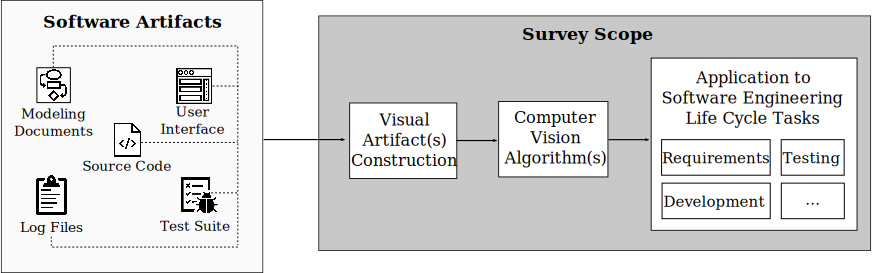
\includegraphics[scale=0.50]{survey/figures/scope-horizontal}
    %}
    \caption{Overview of the scope of this survey.}
    \label{fig:scope}
\end{figure*}






% !TEX root =  manuscript.tex
\section{Conclusions}\label{sec:conclusions}
A recent and growing trend in software engineering 
research is to adopt a \emph{visual perspective} of 
the software, which entails extracting and processing 
\textit{visual artifacts} relevant to the software being analyzed. 
To gain a better understanding of this trend,
in this chapter, we surveyed the literature on the use of 
visual analysis approaches in software engineering. 
From more than \initialPoolSize publications, 
we systematically obtained \numberOfPapers papers 
and analyzed them according to a number of research dimensions.
Our study revealed that visual analysis techniques 
have been utilized in all areas of software engineering, 
albeit more prevalently in the software testing field.
We also discussed why visual analysis was utilized, 
how these techniques are evaluated, and what limitations they bear.
Our suggestions for future work include the development 
of common frameworks and visual benchmarks to collect 
and evaluate the state-of-the-art techniques, 
to avoid relying on ad-hoc solutions. We believe that 
the findings of this work illustrate the potential of 
visual approaches in software engineering, and may help 
newcomers to the field in better understanding the research landscape.

\hl{A number of key findings can be observed from the survey in order to help in 
guiding and framing the remainder of the dissertation. 
First, cross-browser testing is by far the most common area of application, 
whereas exploring non-functional properties received little to no focus. 
This shows that there is an opportunity to explore the use of visual analysis 
in improving non-functional properties, and therefore the remainder of the dissertation 
will be focusing on this aspect. This will provide better and more novel research 
contributions compared to exploring functional properties. 
Furthermore, our survey of the visual analysis techniques used shows that the 
majority of existing works use some form of basic image diffing or features. This shows that it would be novel and potentially useful to investigate more fine-grained level of visual analysis that examines fine-grained visual details. Accordingly, this unexplored approach will be the basis of the techniques proposed in the remainder of the dissertation.}  


\balance


%% !TEX root =  paper.tex

\section*{Acknowledgments}
\label{section:acknowledgments}

\balance
\bibliographystyle{ACM-Reference-Format}
\bibliography{bibliography}

\end{document}


